\documentclass[12pt]{beamer}

\usetheme{Air}
\usepackage{thumbpdf}
\usepackage{wasysym}
\usepackage{ucs}
\usepackage[utf8]{inputenc}
\usepackage{pgf,pgfarrows,pgfnodes,pgfautomata,pgfheaps,pgfshade}
\usepackage{verbatim}

\usepackage[font={small,color=darkgray},labelfont=bf,hypcap=true]{caption}
% does not work in beamer
%\usepackage[font={footnotesize,color=darkgray},labelfont=bf,hypcap=true]{subcaption}

%%%%%%%%%%%%%%%%%%%%%%%%%%%%%%%%%%%%%%%%%%%%%%%%%%%%%%%%
% 
% MATH ONLY
%
%%%%%%%%%%%%%%%%%%%%%%%%%%%%%%%%%%%%%%%%%%%%%%%%%%%%%%%%

% substitute
\usepackage{xstring}
\def\replaceStr#1{%
  \IfSubStr{#1}{,}{%
    \StrSubstitute{#1}{beingSubstituted}{desired}
  }{#1}
}

% Column vectors (any number of arguments)
% gives error in texclipse because of the pmatrix pair!
% \newcount\colveccount
% \newcommand*\colvecn[1]{
%         \global\colveccount#1
%         \begin{pmatrix}
%         \colvecnext
% }
% \def\colvecnext#1{
%         #1
%         \global\advance\colveccount-1
%         \ifnum\colveccount>0
%           \\
%           \expandafter\colvecnext
%         \else
%            \end{pmatrix}
%         \fi
% }
\usepackage{bm}
% ========= Vectors and matrices ===================
%
% Comment out to use arrow as vector notation
\renewcommand{\vec}[1]{\mathbf{#1}}
%\renewcommand{\vec}[1]{\bm{#1}}
%\renewcommand{\vec}[1]{\boldsymbol #1}
\newcommand{\colvec}[1]{\begin{pmatrix} #1 \end{pmatrix}}
% Matrix does not use bold now 
\newcommand{\mat}[1]{#1}
%\newcommand{\mat}[1]{\mathbf{#1}}
% transpose
\newcommand{\trsp}{^T}

% ========== Common sets ===========================
\newcommand{\real}{\mathbb{R}}
\newcommand{\complex}{\mathbb{C}}
\newcommand{\nat}{\mathbb{N}}
\newcommand{\integer}{\mathbb{Z}}

% derivative
\newcommand{\pder}[2]{\frac{\partial#1}{\partial#2}}
\newcommand{\pderop}[1]{\frac{\partial}{\partial#1}}
\newcommand{\der}[2]{\frac{\mathrm{d}#1}{\mathrm{d}#2}}
\newcommand{\derop}[1]{\frac{\mathrm{d}}{\mathrm{d}#1}}
\newcommand{\secpder}[3]{\frac{\partial^2 #1}{\partial #2 \partial #3}}
\newcommand{\npder}[3]{\frac{\partial^{#3} #1}{\partial #2^{#3} }}
\newcommand{\nder}[3]{\frac{\mathrm{d}^{#3} #1}{\mathrm{d} #2^{#3} }}

% equal by definition
\usepackage{mathtools}
\newcommand{\defeq}{\vcentcolon=}

% ============= Norm ==============================
%
% usage: \norm{ \biggl(\sum_{n=1}^N \mathbf{P}_{n}\biggr) }
\newcommand{\norm}[1]{\left\lVert#1\right\rVert}

% ===============Functions ========================
%
% Trigo
%
\newcommand{\sech}{\, \mathrm{sech} \,}
\newcommand{\sinc}{\, \mathrm{sinc} \,}


% math operators
\DeclareMathOperator{\colspan}{colspan}
\DeclareMathOperator{\rank}{rank}
\DeclareMathOperator{\conv2}{\ast\ast}
\DeclareMathOperator{\corr2}{\star\star}
% argmin/max
\DeclareMathOperator*{\argminOp}{argmin}
\DeclareMathOperator*{\argmaxOp}{argmax}
\newcommand*{\argmin}{\argminOp\limits}
\newcommand*{\argmax}{\argmaxOp\limits}

% =================== Fancy =======================
% Fourier transform operator
\DeclareMathOperator{\FT}{\mathfrak{F}}


% \usepackage{enumitem}
% \setlist[itemize,2]{label={$\star$}}

\pdfinfo
{
  /Title       (Image Segmentation based on Wavelet Coefficients)
  /Creator     (TeX)
  /Author      (Rex Ying)
}


\title{Image Segmentation based on Wavelet Coefficients}
\subtitle{Digital Image Processing Final Project}
\author{Rex Ying}
%\date{September 6th 2006}

\begin{document}

\frame{\titlepage}

\section*{}
\begin{frame}
  \frametitle{Outline}
  %\tableofcontents[section=1,hidesubsections]
  \tableofcontents[hidesubsections]
\end{frame}

\AtBeginSection[]
{
  \frame<handout:0>
  {
    \frametitle{Outline}
    \tableofcontents[currentsection,hideallsubsections]
  }
}

\AtBeginSubsection[]
{
  \frame<handout:0>
  {
    \frametitle{Outline}
    \tableofcontents[sectionstyle=show/hide,subsectionstyle=show/shaded/hide]
  }
}

\newcommand{\highlighton}[2]{%
  \alt#2{\structure{#1}}{#1}
}

\newcommand{\highlighttext}[1]{
  \textcolor{airorange}{#1}
}

\newcommand{\icon}[1]{\pgfimage[height=1em]{#1}}



%%%%%%%%%%%%%%%%%%%%%%%%%%%%%%%%%%%%%%%%%
%%%%%%%%%% Content starts here %%%%%%%%%%
%%%%%%%%%%%%%%%%%%%%%%%%%%%%%%%%%%%%%%%%%



\section{Introduction}

\begin{frame}
  \frametitle{Objectives}
  \framesubtitle{types of segmentation}
  \begin{block}{}
  \begin{itemize}
    \item Segmenting textures (possibly noisy)
    \item Properties of textures in general: space invariant, high pass
  \end{itemize}
  \end{block}
  
  \begin{figure}[H]
  \centering
  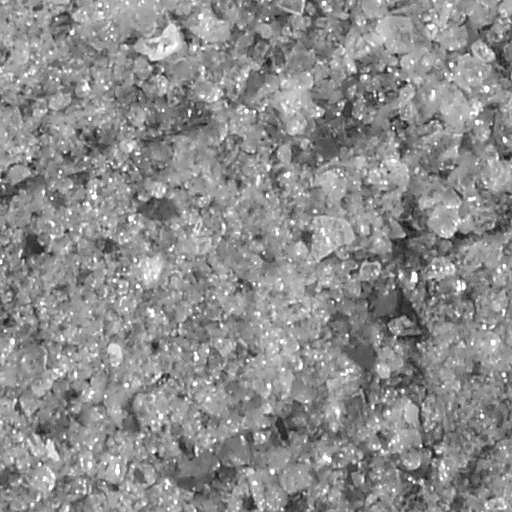
\includegraphics[scale=0.2]{../data/glass/glass1_t0}
  \label{fig:glass_texture}
  \caption{Example of texture }
  \end{figure}
\end{frame}

\begin{frame}
  \frametitle{Prerequisites \& Assumptions}
  \framesubtitle{Discrete Wavelet Transform}
  \begin{block}{Properties of wavelet coefficients}
  \begin{itemize}
    \item Distribution of wavelet coefficients in general is heavily tailed
    \item Heisenberg uncertainty principle: time / frequency tradeoff
    \item Interscale and intrascale relations
  \end{itemize}
  \end{block}
  \begin{figure}[H]
  \centering
  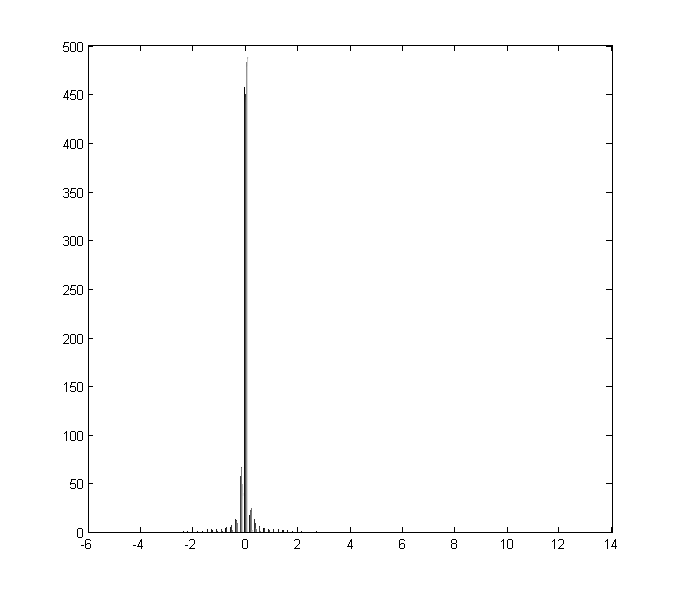
\includegraphics[scale=0.15]{../figs/theory/hist_wavelet_coefs}
  \label{fig:hist_wavelet_coefs}
  \caption{Example of wavelet coefficients distribution}
  \end{figure}
\end{frame}

\section{Theory}
\begin{frame}
  \frametitle{Modeling wavelet coefficients}
  \framesubtitle{Mixed Gaussian}
  
  It is the wavelet coefficient, instead of scaling coefficient, that is of more
  importance.
  \begin{figure}[H]
  \centering
  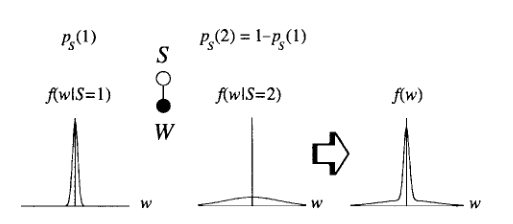
\includegraphics[scale=0.5]{../figs/theory/mixed_gaussian}
  \label{fig:hist_wavelet_coefs}
  \caption{Example of wavelet coefficients distribution}
  \end{figure}
  Parameters:
  $$
    \mu_s, \sigma_s, \mu_l, \sigma_l
  $$
  But why a mixture of TWO Gaussian?
\end{frame}

\begin{frame}
  \frametitle{Determination of parameters}
  \framesubtitle{using information from the entire wavelet tree}
  \begin{block}{Standard block}
  \begin{itemize}
    \item What is tempting: independent assumption
    \item In real world: coefficients are correlated
    \item Markov models
    \begin{itemize}
      \item Markov chains
      \item Markov trees
    \end{itemize}
  \end{itemize}
  \end{block}   
\end{frame}

% \begin{frame}
%   \frametitle{Determination of parameters}
%   \framesubtitle{Notion of dyadic squares}
%   
%   \begin{figure}[h!]
%   \begin{subfigure}[t]{0.4\textwidth}
% 	\centering
% 	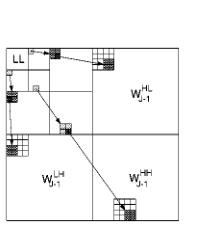
\includegraphics[width=\textwidth]{../figs/theory/wavelet_coefs}
% 	\caption{Wavelet coefficients }
% 	\label{fig:wavelet_coefs}
%   \end{subfigure}
%   \begin{subfigure}[t]{0.4\textwidth}
% 	\centering
% 	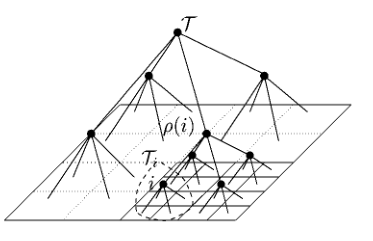
\includegraphics[width=\textwidth]{../figs/theory/wavelet_coefs_tree}
% 	\caption{Tree structure }
% 	\label{fig:wavelet_coefs_tree}
%   \end{subfigure}
%   \end{figure}
%   
% \end{frame}

\begin{frame}
  \frametitle{Determination of parameters}
  \framesubtitle{using information from the entire wavelet tree}

  \begin{figure}[H]
  \centering
  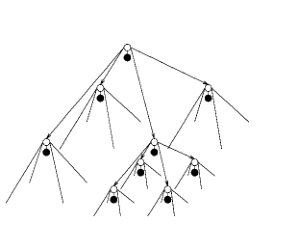
\includegraphics[scale=0.7]{../figs/theory/hmt}
  \label{fig:hmt}
  \caption{Hidden Markov Tree}
  \end{figure} 
\end{frame}

\begin{frame}
  \frametitle{Determination of parameters}
  \framesubtitle{using information from the entire wavelet tree}
  
  \begin{alertblock}{Very important assumption}
  \begin{itemize}
    \item The state ($s$ or $l$) directly determines the distribution of coefficients.
    \item The states are correlated across scale, NOT the wavelet coefficients.
    \item Given the state, the subtree rooted at a node of the tree is independent from
    the rest of the tree
  \end{itemize}  	
  \end{alertblock}
 
\end{frame}

\begin{frame}
  \frametitle{Hidden Markov Tree Model}
  \framesubtitle{Parameters}
  
  \begin{block}{Very important assumption}
  \begin{itemize}
    \item $\epsilon^{\rho(i), m}_{i, n} $: conditional probability $P(S(i) = n |
    S(\rho(i)) = m)$ The transition stochastic matrix (properties?):
     $$ \begin{bmatrix}
       \epsilon^{\rho(i), s}_{i, s} & 1 - \epsilon^{\rho(i), s}_{i, s} \\
       1 - \epsilon^{\rho(i), l}_{i, l} & \epsilon^{\rho(i), l}_{i, l}
     \end{bmatrix} $$
    \item ${P_S}_i(m) = P(S(i) = m)$: state probabilities
    \item $\mu_i(m)$: mean of Gaussian in state $m$
    \item $\sigma_i(m)$: standard deviation of Gaussian in state $m$
  \end{itemize}  	
  \end{block}
\end{frame}
  
\begin{frame}
  \frametitle{Hidden Markov Tree Model}
  \framesubtitle{Within and between wavelet tree tying}
  
  \begin{block}{Tying}
  \begin{itemize}
    \item Noise
    \item A huge number of wavelet coefficients
    \item Overfitting and robustness
    \item On the same level, $3$ sets of coefficients would suffice
  \end{itemize}  	
  \end{block}
 
\end{frame}

\section{Technical aspects}
\begin{frame}
  \frametitle{Choice of wavelet}

  \begin{block}{A desired wavelet}
  An ``eligible'' wavelet should at least have the property of detecting edges.
  \begin{itemize}
    \item Haar
    \item Daubechies 4-tap wavelet
    \item Gabor wavelet
  \end{itemize}
  \end{block}
\end{frame}

\newcommand{\putlink}[1]{%
   \pgfsetlinewidth{1.4pt}%
   \pgfsetendarrow{\pgfarrowtriangle{4pt}}%
   \pgfline{\pgfxy(1,1)}{\pgfxy(#1,1)}
}

\begin{frame}
  \frametitle{Steps}
  
  \begin{block}{Time bomb}
%   \begin{enumerate}
%     \item<2-> Two more to go
%     \item<3-> One more to go
%     \item<4-> Last chance...
%     \item<5-> BOOM!
%   \end{enumerate}
   \begin{enumerate}
    \item Training using labeled data (images) to obtain the HMT model \pause
    \item Find the likelihood of the image given models for each texture \pause
    \item Optimization techniques (inter and intra-scale fusion) \pause
  \end{enumerate}
  \end{block}
\end{frame}

\begin{frame}
  \frametitle{Training}
  \framesubtitle{Expectation maximization algorithm}
  
  \begin{block}{Rationale}
    \begin{itemize}
      \item Iterative methods
	  \item Jensen's inequality
	  \item Arithmetic-geometric inequality
	  \item Maximize log-likelihood $L(\theta) = \ln P(\vec{X} | \theta)$
	\end{itemize}
  \end{block}
  
  \begin{align*}
    & L(\theta) - L(\theta_n) = \ln \sum_\vec{z} P(\vec{X} | \vec{z}, \theta) P(\vec{z} |
    \theta) - \ln P(\vec{x} | \theta) \\
    & L(\theta) - L(\theta_n) \ge \sum_\vec{z} P(\vec{z} | \vec{X}, \theta_n) \ln \left(
    \frac{P(\vec{X} | \vec{z}, \theta) P(\vec{z} | \theta)}{P(\vec{z} | \vec{X}, \theta_n)
    P(\vec{X} | \theta_n)} \right)
  \end{align*}
\end{frame}

\begin{frame}
  \frametitle{Training}
  \framesubtitle{Expectation maximization algorithm}
  
  A fixed point iteration:
  \begin{align*}
    & L(\theta_n) + \Delta(\theta_n | \theta_n) = L(\theta_n)
  \end{align*}
  \begin{figure}[H]
  \centering
  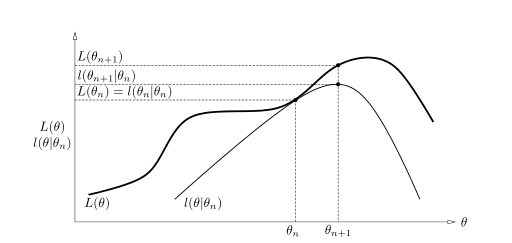
\includegraphics[scale=0.7]{../figs/theory/em_graph_interpretation}
  \label{fig:em_graph_interpretation}
  \caption{Graphical interpretation of EM}
  \end{figure} 
\end{frame}

\begin{frame}
  \frametitle{Training}
  \framesubtitle{Expectation maximization algorithm}
  
  \begin{block}{EM steps}
    Expectation step:
    $$ P(\vec{S} | \vec{w}, \bm{\theta}_k) $$
    $$ P(S_i = m, \mathcal{T}_1 | \theta) = P(\mathcal{T}_i | S(i) = m, \bm{\theta})
    \times P(\mathcal{T}_{1 \backslash i}, S(i) = m | \bm{\theta})
    $$
    Multitree\ldots
    
    \pause
    Maximization step: (amazingly it is easier)
    $$ \argmax_{\bm{\theta}} E_S \left[ \ln P(\vec{w}, \vec{S} | \bm{\theta}) |
    \vec{w}, \bm{\theta}_k \right] $$
    
    \pause
    Increment $k$, until convergence.
  \end{block}
\end{frame}

\section{Performance}
\begin{frame}
  \frametitle{Data}
  \framesubtitle{Types of textures}
  
  \begin{figure}[H]
  \centering
  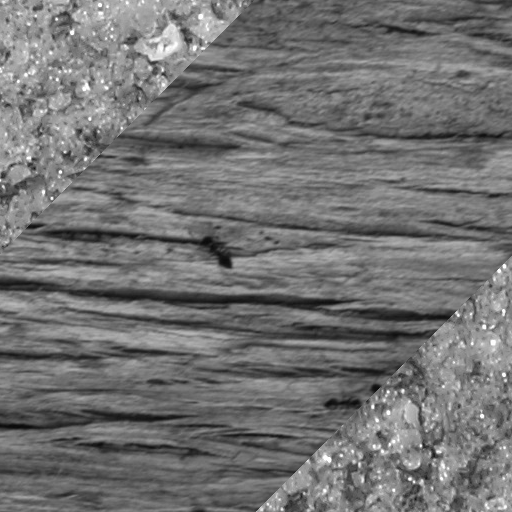
\includegraphics[scale=0.3]{../data/mytest/test1}
  \label{fig:test1}
  \caption{A test image}
  \end{figure} 
  
\end{frame}

\begin{frame}
  \frametitle{Data}
  \framesubtitle{Types of textures}
  
  \begin{figure}[H]
  \centering
  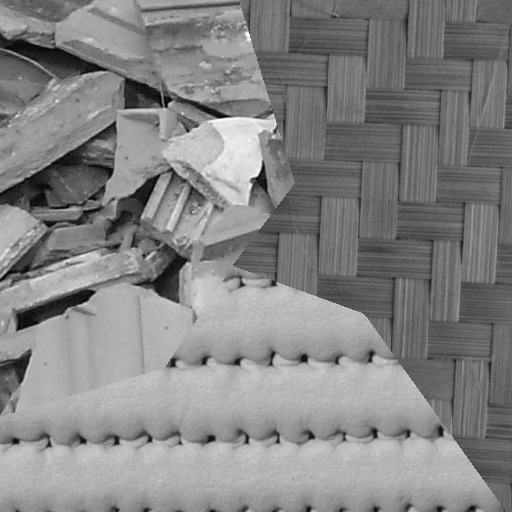
\includegraphics[scale=0.3]{../data/tm1_1_1}
  \label{fig:tm1_1_1}
  \caption{A test image}
  \end{figure} 
  
\end{frame}

\begin{frame}
  \frametitle{Result}
  \framesubtitle{Raw segmentation}
  
  \begin{figure}[H]
  \centering
  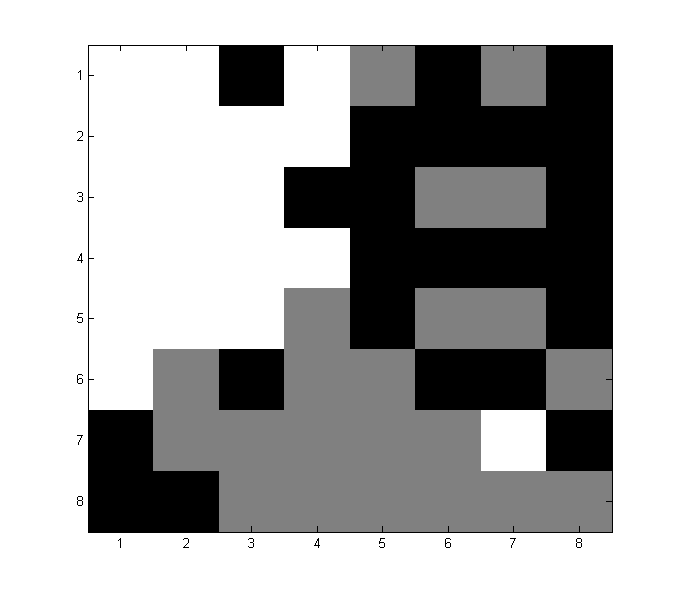
\includegraphics[scale=0.3]{../figs/raw_seg_k=4}
  \label{fig:tm1_1_1}
  \caption{Raw segmentation at 16-by-16 dyadic squares}
  \end{figure} 
  
\end{frame}

\begin{frame}
  \frametitle{Result}
  \framesubtitle{Raw segmentation}
  
  \begin{figure}[H]
  \centering
  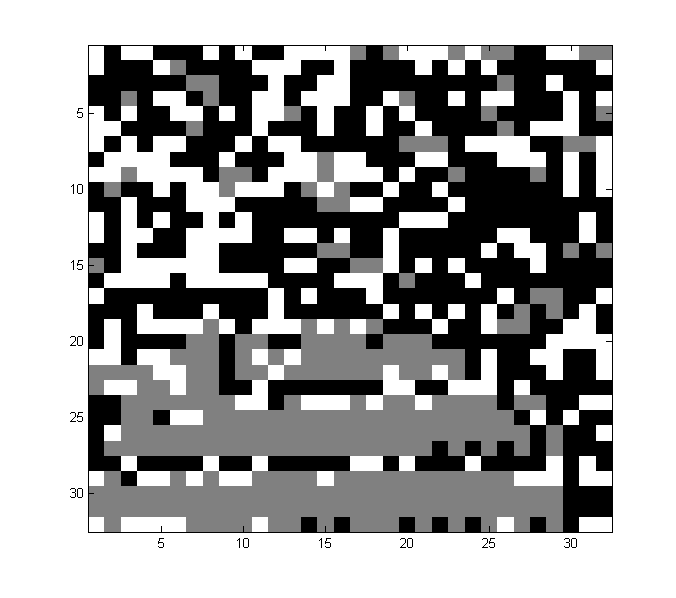
\includegraphics[scale=0.3]{../figs/raw_seg_k=7}
  \label{fig:tm1_1_1}
  \caption{Raw segmentation at 2-by-2 dyadic squares}
  \end{figure} 
  
\end{frame}

\begin{frame}
  \frametitle{Result}
  \framesubtitle{Segmentation after fusion}
  
  \begin{figure}[H]
  \centering
  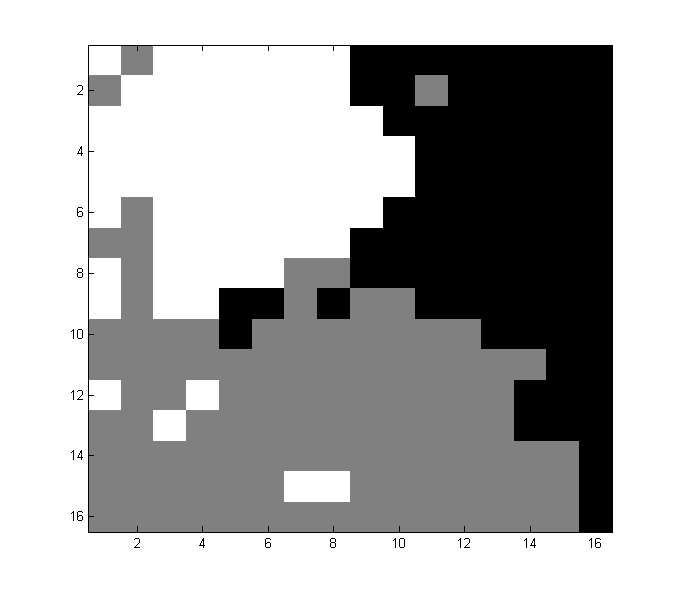
\includegraphics[scale=0.3]{../figs/fused_seg_k=5}
  \label{fig:tm1_1_1}
  \caption{Raw segmentation at 2-by-2 dyadic squares}
  \end{figure} 
  
\end{frame}

\begin{frame}
  \frametitle{Deal with noise}
  \framesubtitle{HMT denoising}
  
  \begin{figure}[H]
  \centering
  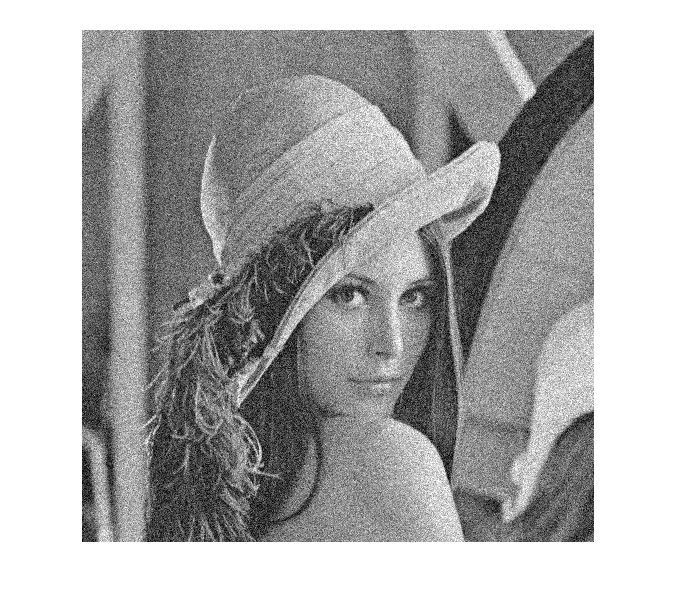
\includegraphics[scale=0.35]{../figs/lena_noisy}
  \label{fig:lena_noisy}
  \caption{Noisy Lena}
  \end{figure} 
\end{frame}

\begin{frame}
  \frametitle{Deal with noise}
  \framesubtitle{HMT denoising}
  
  \begin{figure}[H]
  \centering
  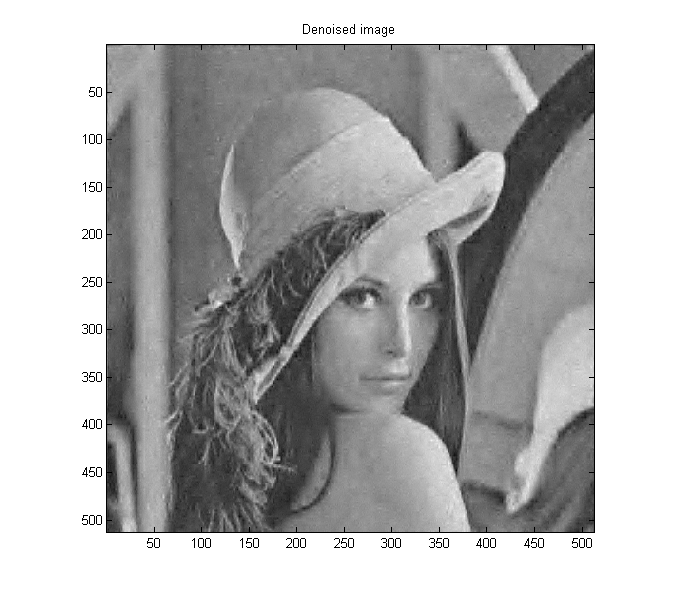
\includegraphics[scale=0.35]{../figs/lena_denoised_hmt}
  \label{fig:lena_denoised_hmt}
  \caption{Denoised using HMT}
  \end{figure} 
\end{frame}

\begin{frame}
  \frametitle{Deal with noise}
  \framesubtitle{HMT denoising}
  \begin{figure}[H]
  \centering
  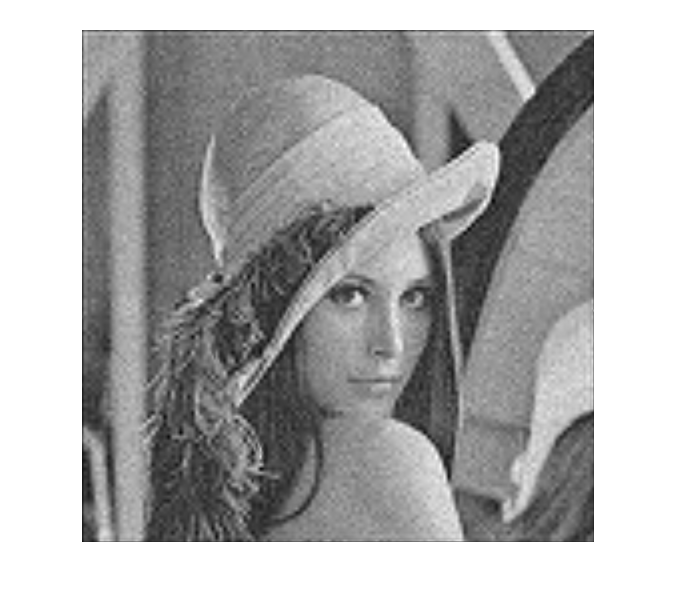
\includegraphics[scale=0.35]{../figs/lena_denoised_wavelet_thresholding}
  \label{fig:lena_denoised_wavelet_thresholding}
  \caption{Denoised by applying Donoho-Johnstone universal threshold on wavelet
  coefficients}
  \end{figure} 
\end{frame}

\begin{frame}
  \frametitle{Deal with noise}
  \framesubtitle{HMT denoising}
  
  \begin{figure}[H]
  \centering
  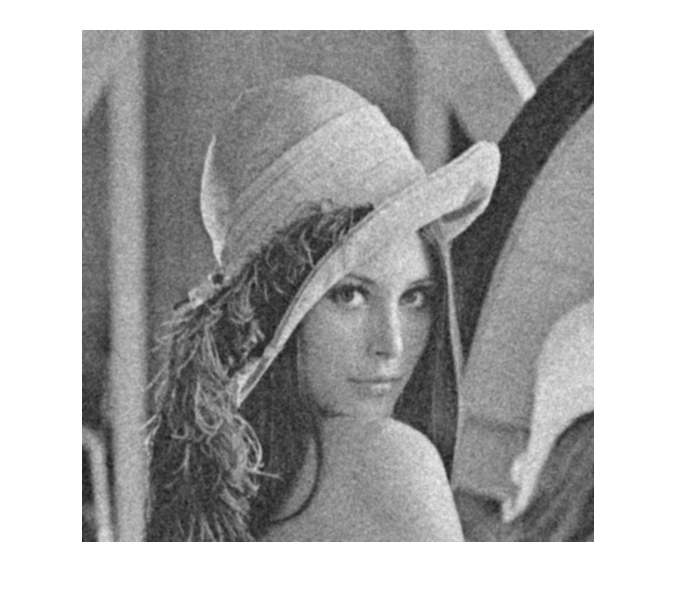
\includegraphics[scale=0.35]{../figs/lena_denoised_gaussian}
  \label{fig:lena_denoised_gaussian}
  \caption{Denoised using Gaussian kernel}
  \end{figure} 
\end{frame}

\section*{}
\frame{
  \vfill
  \centering
  \highlighton{
  \usebeamerfont*{frametitle} So\ldots

  \usebeamerfont*{framesubtitle} This project involves quite a number of things that I
  have not touched }
  \vfill
}
\begin{frame}
  \frametitle{Other aspects, TODOs }
  
  \begin{example}
    \begin{itemize}
    \item single pixel level segmentation
    \item Inter and intra-scale fusion
    \item Choice of wavelet levels
  \end{itemize}
  \end{example}

  \begin{block}{TODO}
  \begin{itemize}
    \item A better understanding of performance limitations
    \item Investigate effects of different wavelet basis representations
    \item Nice procedure for segmenting noisy images
    \item Combination with other segmentation techniques
  \end{itemize}
  \end{block}
\end{frame}

\begin{frame}
  \frametitle{Further exploration }
  \begin{block}{Further exploration}
  \begin{itemize}
    \item Better scheme for choosing wavelet levels
    \item Un-supervised learning
    \item Analysis of multiscale classification errors
  \end{itemize}
  \end{block}
\end{frame}

\frame{
  \vspace{2cm}
  {\huge Questions ?}

  \vspace{3cm}
  \begin{flushright}
    Rex Ying

    \structure{\footnotesize{zy26@duke.edu}}
  \end{flushright}
}

\end{document}
